%:
% !TEX TS-program = pdflatex
% !TEX encoding = UTF-8 Unicode

% This is a simple template for a LaTeX document using the "article" class.
% See "book", "report", "letter" for other types of document.

%\documentclass{scrartcl}
\documentclass[11pt]{report} % use larger type; default would be 10pt
%\setkomafont{disposition}{\normalfont\bfseries}	

\usepackage[utf8]{inputenc} % set input encoding (not needed with XeLaTeX)

%%% PAGE DIMENSIONS
\usepackage{geometry} % to change the page dimensions
\usepackage{amsmath}
\geometry{a4paper} % or letterpaper (US) or a5paper or....
% \geometry{margin=2in} % for example, change the margins to 2 inches all round
% \geometry{landscape} % set up the page for landscape
%   read geometry.pdf for detailed page layout information

\usepackage{booktabs}% http://ctan.org/pkg/booktabs

\usepackage{graphicx} % support the \includegraphics command and options
\usepackage{natbib} % support the \includegraphics command and options
\usepackage{xcolor,colortbl}

\usepackage{multicol}

% \usepackage[parfill]{parskip} % Activate to begin paragraphs with an empty line rather than an indent

%%% PACKAGES
\usepackage{booktabs} % for much better looking tables
\usepackage{array} % for better arrays (eg matrices) in maths
\usepackage{paralist} % very flexible & customisable lists (eg. enumerate/itemize, etc.)
\usepackage{verbatim} % adds environment for commenting out blocks of text & for better verbatim
\usepackage{subfigure} % make it possible to include more than one captioned figure/table in a single float
% These packages are all incorporated in the memoir class to one degree or another...

%%% HEADERS & FOOTERS
\usepackage{fancyhdr} % This should be set AFTER setting up the page geometry
\pagestyle{fancy} % options: empty , plain , fancy
\renewcommand{\headrulewidth}{0pt} % customise the layout...
\lhead{}\chead{}\rhead{}
\lfoot{}\cfoot{\thepage}\rfoot{}

%%% SECTION TITLE APPEARANCE
\usepackage{sectsty}
\allsectionsfont{\sffamily\mdseries\upshape} % (See the fntguide.pdf for font help)
% (This matches ConTeXt defaults)

%%% ToC (table of contents) APPEARANCE
\usepackage[nottoc,notlof,notlot]{tocbibind} % Put the bibliography in the ToC
\usepackage[titles,subfigure]{tocloft} % Alter the style of the Table of Contents
\renewcommand{\cftsecfont}{\rmfamily\mdseries\upshape}
\renewcommand{\cftsecpagefont}{\rmfamily\mdseries\upshape} % No bold!

\newcommand{\sw}{\textit{software}\xspace}
\newcommand{\Sw}{\textit{Software}\xspace}
\newcommand{\sws}{\textit{softwares}\xspace}
\newcommand{\iso}{ISO 29110\xspace}
\newcommand{\dsw}{Desenvolvimento de \Sw}

\newcommand{\gp}{Gerente de Projeto\xspace}
\newcommand{\kick}{reunião de \textit{kick-off} do projeto\xspace}
\newcommand{\Kick}{Reunião de \textit{kick-off} do projeto\xspace}
\newcommand{\stake}{\textit{stakeholders}\xspace}
\newcommand{\bline}{\textit{baseline}\xspace}

\newcommand{\amb}{Fatores Ambientais\xspace}
\newcommand{\ativ}{Ativos de Processos Organizacionais\xspace}

% nomenclaturas de documentação
\newcommand{\planproj}{Plano de Gerenciamento do Projeto\xspace}
\newcommand{\planesc}{Plano de Gerenciamento do Escopo\xspace}
\newcommand{\plancron}{Plano de Gerenciamento do Cronograma\xspace}
\newcommand{\plancusto}{Plano de Gerenciamento de Custos\xspace}
\newcommand{\planqual}{Plano de Gerenciamento da Qualidade\xspace}
\newcommand{\planpess}{Plano de Gerenciamento de Pessoal\xspace}
\newcommand{\plancom}{Plano de Gerenciamento das Comunicações\xspace}
\newcommand{\planrisco}{Plano de Gerenciamento de Riscos\xspace}
\newcommand{\planaq}{Plano de Gerenciamento de Aquisições\xspace}

\newcommand{\termo}{Termo de Abertura do Projeto\xspace}

\newcommand{\bok}{Guia PMBOK$^{\small{\textregistered}}$\xspace}

\newcommand{\msp}{Project\xspace}

\usepackage{titling}
\usepackage[brazil]{babel}
\usepackage{xspace}

\usepackage{framed}

\usepackage{setspace}
\onehalfspacing

\usepackage{url}

%\DeclareUnicodeCharacter{00A0}{ }

%%% END Article customizations

%%% The "real" document content comes below...

\begin{document}

%\inputencoding{latin1}\input{titulo}
% !TEX root = Apostila GP.tex

\chapter{Fundamentos}

O Guia do Conhecimento em Gerenciamento de Projetos (\bok) é uma norma reconhecida para a profissão de gerenciamento de projetos. Um padrão é um documento formal que descreve normas, métodos, processos e práticas estabelecidas. Assim como em outras profissões como advocacia, medicina e contabilidade, o conhecimento contido nesse padrão evoluiu a partir das boas práticas reconhecidas de profissionais de gerenciamento de projetos que contribuíram para o seu desenvolvimento.
% !TEX root = Apostila GP.tex

\chapter{Gerenciamento de Integração}

\begin{figure}[!h]
\centering
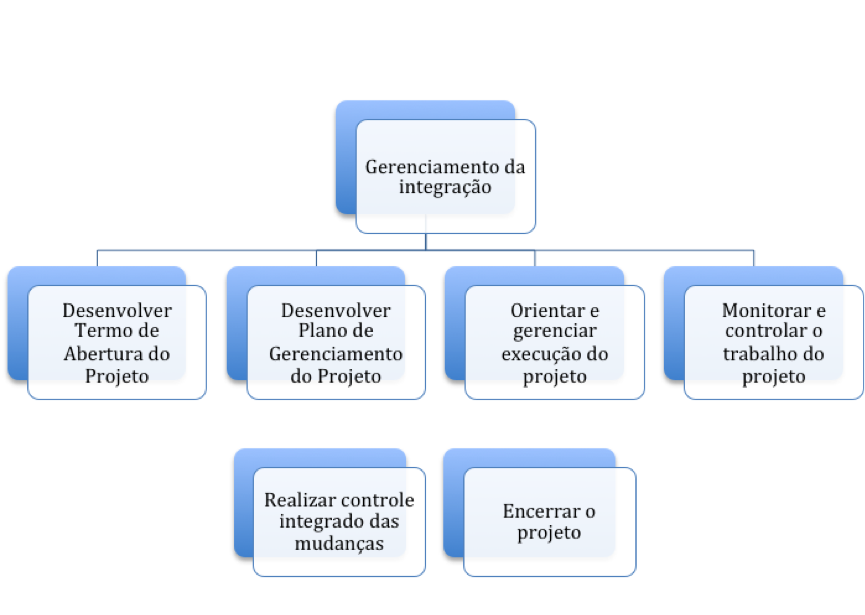
\includegraphics[scale=0.75]{Figuras/gerenciamento_integracao.png}
\caption{Processos do Gerenciamento da Integração}
\label{fig:proc:ger:integr}
\end{figure}

\section{\planproj}

O \planproj é um documento usado no auxílio da gerência do projeto no seu dia a dia. Ele é formalizado e aprovado pelos \stake e deve conter informações realistas sobre o projeto.

Ele é composto por:

\begin{itemize}

\item Plano do planejamento

\item Planos de gerenciamento de todas as áreas que serão controladas

\item Linha de base do escopo, cronograma e orçamento

\item Outros documentos e processos importantes para o gerenciamento do projeto

\end{itemize}

\subsection{Plano do planejamento}

É considerado como o pré-planejamento. Consiste em atribuir datas, responsáveis e tarefas com o objetivo de planejar o projeto e gerar os documentos e informações necessárias para a \kick. A Figura \ref{fig:plano:planejamento} mostra um exemplo de plano contendo algumas das tarefas mais importantes.

\begin{figure}[!h]
\centering
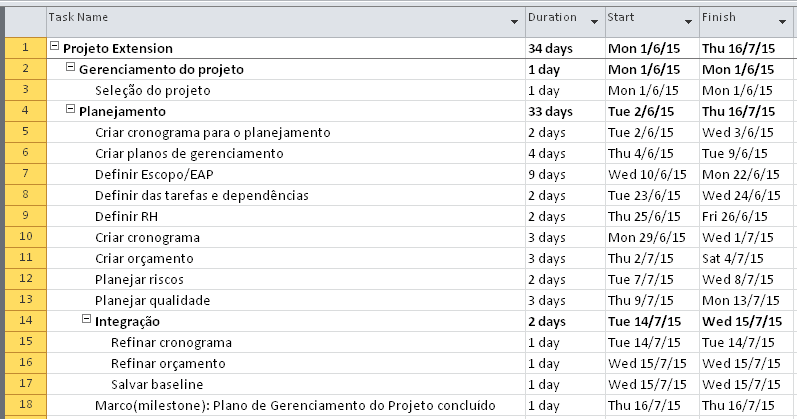
\includegraphics[scale=0.5]{Figuras/plano_planejamento.png}
\caption{Exemplo de Plano do Planejamento}
\label{fig:plano:planejamento}
\end{figure}

\subsection{\Kick}

É o evento que formaliza o início do projeto e que tem como um dos objetivos principais deixar claro os papéis e responsabilidades de todos no projeto. Por isso a participação de todos os \stake é de suma importância. Trata-se de uma ótima oportunidade de colocar frente a frente a equipe, clientes e outros \stake.

\subsection{Integracão dos planos}

Um projeto é como um organismo vivo no qual uma deficiência em uma área pode influenciar uma ou mais outras áreas. Quanto mais tarde essa deficiência for detectada e corrigida, piores serão as consequências.

Por este motivo, os planos de gerenciamento das diversas áreas do projeto não podem ser considerados totalmente independentes e devem ser construídos e mantidos de forma integrada.

Os planos de gerenciamento do projeto seguem as áreas de conhecimento que serão estudadas:

\begin{itemize}

\item \planesc
\item \plancron
\item \plancusto
\item \planqual
\item \planpess
\item \plancom
\item \planrisco
\item \planaq

\end{itemize}

Organizações que possuem escritórios de projeto (PMO) podem definir planos de gerenciamentos padronizados para que não se perca tempo com processos que se repetem em cada novo projeto. Neste caso, cabe ao \gp seguir os processos e planos definidos e o Plano do Planejamento vai incluir somente o cronograma das etapas.

\subsection{Processo Desenvolver o \planproj}

\begin{figure}[!h]
\centering
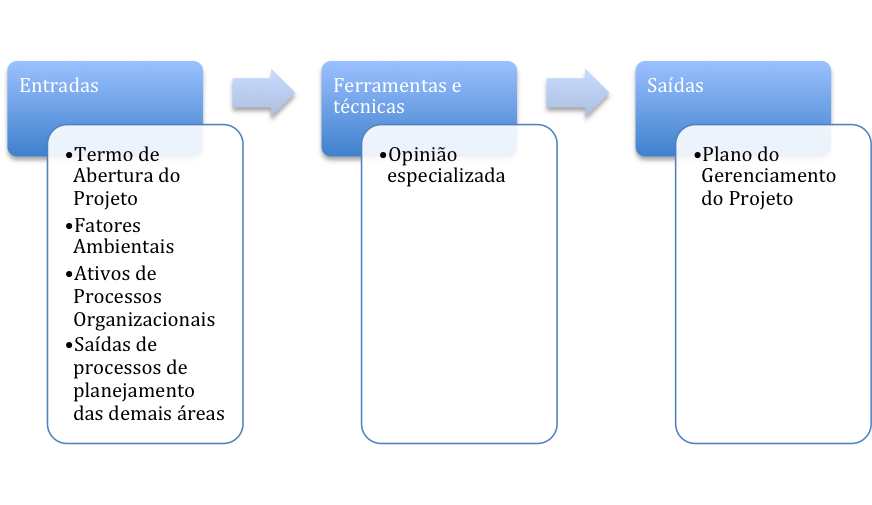
\includegraphics[scale=0.75]{Figuras/proc_integracao_1.png}
\caption{Processo Desenevolver o \planproj}
\label{fig:proc:des:planproj}
\end{figure}

\subsubsection{Entradas}

\begin{itemize}

\item \termo: principal base para início do planejamento, pois possui tudo que ja foi definido para o projeto até o momento.

\item \amb: cultura, infraestrutura, mercado, normas, etc.

\item \ativ: processos e métodos pré-definidos, informações históricas, lições aprendidas, etc.

\item Saidas de processos de planejamento das demais áreas: geram documentos e informações que devem ser integradas para a criação do \planproj. Alterações nestes planos geram alterações no \planproj.

\end{itemize}

\subsubsection{Ferramentas e técnicas}

Opinião especializada:

\begin{itemize}

\item Entender as necessidades do projeto e customizar os processos de acordo

\item Desenvolver e incluir no \planproj detalhes de nível técnico ou gerencial

\item Determinar recursos e conhecimentos necessários para execução do \planproj.

\item Identificar quais documentos necessitam de um processo formal de controle de mudanças.

\end{itemize}

\subsubsection{Saídas}

\planproj.

\subsection{Conteúdo do \planproj}

Além dos demais planos de gerenciamento, o \planproj deve definir:

\begin{itemize}

\item Controle de criação de documentos: quais documentos são necessários, quem tem a responsabilidade de criá-los e quando.

\item Planos auxiliares para gerenciamento das áreas de conhecimento.

\item Linhas de base do escopo, tempo e custo e a formalização dos processos de mudança dessas linhas de base.

\item Processo de controle de mudança:

	\begin{itemize}

	\item Pessoas autorizadas a requisitar mudanças.

	\item Processo de solicitação de mudanças.

	\item Fluxo/processo da mudança:

		\begin{itemize}

		\item Recepção
		\item Análise/avaliação
		\item Classificação
		\item Aprovação
		\item Priorização

		\end{itemize}

\end{itemize}

\end{itemize}

% !TEX root = Apostila GP.tex

\chapter{Gerenciamento do Escopo}

\section{O que é escopo}

Segundo \cite{pmbok}, escopo  é  todo  o  trabalho,  e  somente  o  trabalho  necessário  para  que  o  produto  ou 
serviço objetivo do projeto seja entregue ao seu final.

Esse é o \textbf{Escopo do projeto} que não deve ser confundido com o \textbf{Escopo do produto}, que são os atributos, funcionalidades e características que devem estar presentes no produto ou serviço criado pelo projeto, conforme podemos observar na Figura \ref{fig:escopo:proj:prod}.

\begin{figure}[!h]
\centering
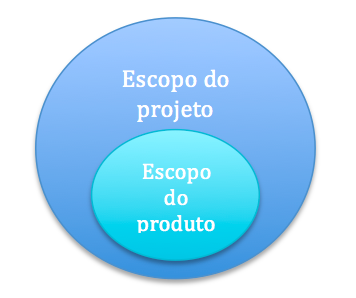
\includegraphics[scale=0.5]{Figuras/escopo_proj_prod.png}
\caption{Escopo produto X escopo projeto}
\label{fig:escopo:proj:prod}
\end{figure}

\section{Gerenciamento do Escopo}

Sãos os processos que visam garantir que o projeto inclua todo o trabalho necessários para completar com sucesso o projeto.

Para isso, deve incluir:

\begin{itemize}

\item Definir e controlar o que \textbf{faz} e o que \textbf{não faz} parte do projeto.

\item Controlar se todo o trabalho está sendo realizado.

\item Controlar o processo de mudanças do escopo.

\item Confrontar as mudanças com o \termo.

\item Evitar retrabalho ou trabalho desnecessário e seus custos

\end{itemize}

\section{Processos}

Para garantir a gerência do escopo, são necessários os seguintes processos:

\begin{itemize}

\item \textbf{Coleta de requisitos}: definir e documentar o que é necessário para se alcançar os objetivos do projeto.

\item \textbf{Definição do escopo}: descrição detalhada do projeto e do produto.

\item \textbf{Criação da Estrutura Analítica do Projeto (EAP)}: a fim de facilitar o gerenciamento das entregas e do trabalho, o escopo deve ser dividido em partes menores e estruturadas.

\item \textbf{Verificação do escopo}: formalizar a aceitação das entregas finalizadas do projeto.

\item \textbf{Controle do escopo}: monitorar e gerenciar o andamento e as mudanças na linha de base do escopo.

\end{itemize}

Os processos dentro do ciclo de vida do projeto podem ser observados na Figura \ref{fig:ciclo:vida}.

\begin{figure}[!h]
\centering
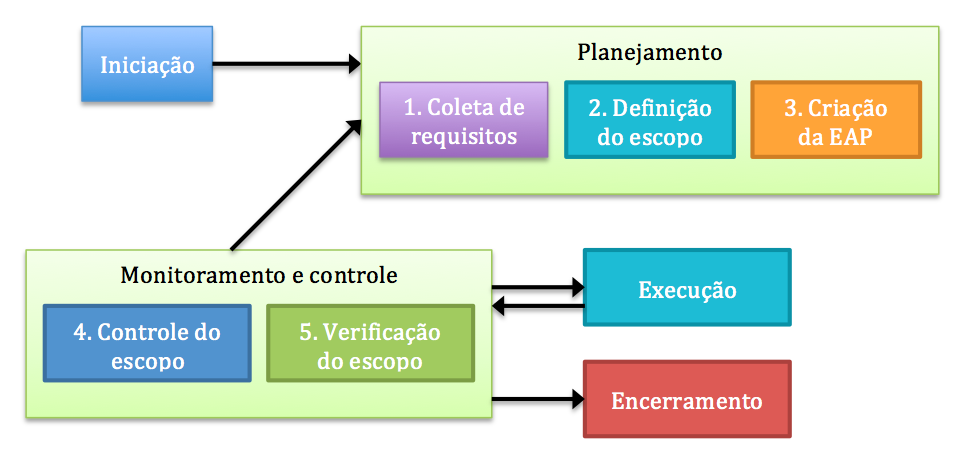
\includegraphics[scale=0.5]{Figuras/ciclo_vida.png}
\caption{Processos dentro do ciclo de vida do projeto}
\label{fig:ciclo:vida}
\end{figure}

\subsection{Inimigos do escopo}

Um escopo com problemas pode levar o projeto ao seu fim. Por isso é importante observar os dois principais inimigos do escopo:

\begin{itemize}

\item \textbf{\textit{Scope Creep}}: aumento do escopo sem nenhum controle, de maneira contínua, muitas vezes de forma lenta, que resulta em um escopo ``inchado'', ingerenciável, cujo foco foge da ideia inicial do projeto e o resultado reflete no aumento dos custos e perda de prazos.

\item \textbf{\textit{Gold Plating}}: adicionar elementos não especificados nos requisitos do projeto, geralmente partindo de equipes técnicas e de desenvolvimento sob a alegação de agregar valor mas cujo resultado é o aumento de custos, perda de qualidade e aumento desnecessário da complexidade do produto.

\end{itemize}

\subsection{Requisitos}

São condições ou capacidades que devem ser supridas pelo resultado do projeto (produto ou serviço) a fim de satisfazer um contrato ou outro documento formal.

São dividos em:

\begin{itemize}

\item \textbf{Requisitos funcionais:} o que o produto ou serviço deve \textbf{fazer}.

\item \textbf{Requisitos não-funcionais:} o que o produto ou serviço deve \textbf{ter}.

\end{itemize}

% !TEX root = Apostila GP.tex

\capitulo{Tempo}

Para gerenciramos o tempo, é preciso primeiramente termos o escopo bem definido, pois o último é base para o primeiro.

\section{Definir atividades}

A partir da EAP vamos traçar a fronteira entre o escopo e o tempo. Isso é feito através da definição das atividades.

Escopo é \textbf{o que} o projeto vai entregar. As atividades são o \textbf{como}, ou seja, de que forma o projeto vai realizar as entregas. A Tabela \ref{tab:ativ:ex} traz alguns exemplos de atividades associadas ao escopo.

\begin{table}[h!]\footnotesize
\centering
\begin{tabular}
{
 	|p{1,8cm}
	| >{\centering\arraybackslash}p{4,9cm}|
}

	\hline

	\multicolumn{2}{c}{Projeto ``Cadeira''}\\
	
	\hline
	
	Escopo&
	Atividade\\
	
	\hline

	Braço&
	\begin{itemize}
		\item Cortar madeira
		\item Lixar
		\item Colar
		\item Envernizar
	\end{itemize}\\
	
	\hline

	Assento&
	\begin{itemize}
		\item Cortar pano
		\item Cortar espuma
		\item Costurar
	\end{itemize}\\

	\hline

\end{tabular}
\caption {Exemplo de lista de atividades}
\label{tab:ativ:ex}
\end{table}

\section{Sequenciar atividades}

Sequenciar é definir a ordem e também as dependências das atividades.

\section{Estimar os recursos das atividades}

Quais os recursos materiais, humanos e tecnológicos que serão necessários para executar cada uma das atividades?

\section{Estimar as durações das atividades}

Quanto tempo será necessário para se concluir cada uma das atividades?

\section{Desenvolver o cronograma}

Um cronograma deve conter:

\begin{itemize}

\item A EAP associada à lista de atividades;

\item O sequenciamento das atividades;

\item Os recursos estimados;

\item As durações estimadas das atividades;

\item As datas reais de início e fim das atividades.

\end{itemize}

A Figura \ref{fig:ativ:ex} traz um exemplo de crongrama contendo todos os elementos citados acima.

\begin{figure}[!h]
\centering
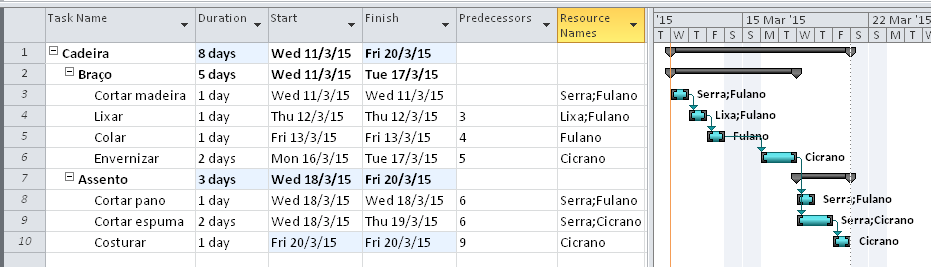
\includegraphics[scale=0.45]{Figuras/ativ_exemplo.png}
\caption{Exemplo de cronograma}
\label{fig:ativ:ex}
\end{figure}
% !TEX root = Apostila GP.tex

\chapter{Ferramentas de TI}

\section{Microsoft Project}

Um dos \sws mais conhecidos de gerenciamento de projetos, se destaca pela sua facilidade de utilização. Aqui apresentaremos algumas das principais funcionalidades da versão 2010.

\subsection{Primeiros passos}

Ao entrar pela primeira vez no \msp, você irá visualizar o modo padrão de exibição, chamado de diagrama de Gantt, pronto para receber dados de seu projeto, conforme as Figuras \ref{fig:msp:tela1} e \ref{fig:msp:tela2}.

\begin{figure}[!h]
\centering
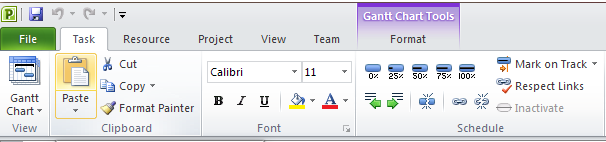
\includegraphics[scale=0.45]{Figuras/project_inicio1.png}
\caption{Guias de comandos e opções do \msp}
\label{fig:msp:tela1}
\end{figure}

\begin{figure}[!h]
\centering
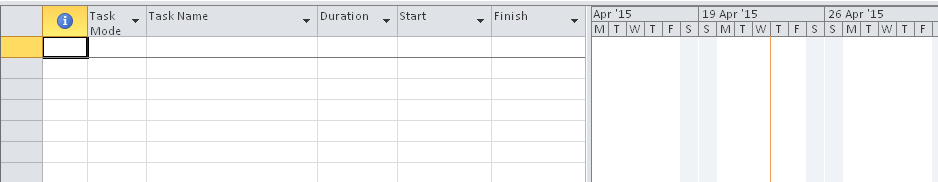
\includegraphics[scale=0.45]{Figuras/project_inicio2.png}
\caption{Tarefas e cronograma do \msp}
\label{fig:msp:tela2}
\end{figure}

Além do modo padrão de exibição, é possível escolher entre outros diversos modos e até mesmo criar o seu próprio modelo. Para isso, basta clicar no botão Gantt Chart (Figura \ref{fig:msp:tela3}) e selecionar um dos modos disponíveis.

\begin{figure}[!h]
\centering
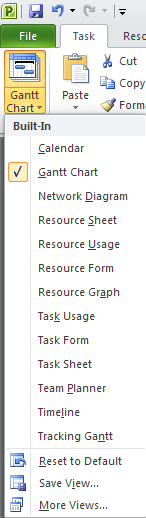
\includegraphics[scale=0.55]{Figuras/project_inicio3.png}
\caption{Botão para troca de modo de visualização}
\label{fig:msp:tela3}
\end{figure}


%\bibliographystyle{plain}
%\bibliographystyle{bibstyle/latex8}     
%\bibliographystyle{apalike-url}     


\bibliographystyle{Bibliografia/apalike-pt}     

%\bibliographystyle{lastchecked}     
            
\bibliography{Bibliografia/research}

\end{document}